\documentclass[11pt,a5paper]{article}
\usepackage[utf8]{inputenc}
\usepackage[english]{babel}
\usepackage{amsmath}
\usepackage{amsthm}
\usepackage{amsfonts}
\usepackage[margin=0.47in]{geometry}
\usepackage{graphicx}

\newtheorem{theorem}{Example}
\newtheorem{exercise}{Exercise}
\newtheorem*{Theorem}{Theorem}

\title{\textbf{Geometry II.}}
\date{Week 9}
\author{Miroslav Stankovic\\ Marko Puza}
\begin{document}
\maketitle

\section{Theory}
After having looked into angle-chasing problem solving approaches in geometry last week, the following pages contain simple tools that will enable us to augment angle-chasing with algebraic tools.\\
More precisely, we will try to reason about angles using lengths and vice versa using Power of a point and Radical lines.

\begin{Theorem}[Power of a point]
Let $s$ denote distance of point $P$ from center $O$ of a circle $k$ with radius $r$. The \emph{Power of a point} with respect to $k$ is a real number $h$ defined as: \[h = s^2 - r^2\]
This number reflects the relative distance of $P$ from $k$. \\
Furthermore, let an arbitrary line through $P$ intersect $k$ in (not necessarily distinct) points $X, Y$. Then \[|PX|\cdot|PY| = h\]
\end{Theorem}

\begin{figure}[h] \begin{center}
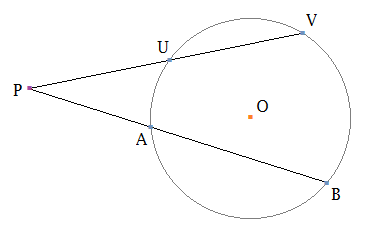
\includegraphics[width=0.5\textwidth]{power}
\caption{Here, $|PA|\cdot|PB| = |PU|\cdot|PV| = h$}
\end{center} \end{figure}

\begin{proof}
We will prove only the case where the point lies outside of a circle - other cases can be proved analogically using similar tirangles.
Consider line through $P$ that intersects circle $k$ in points $X, Y$ and point $T$ also on $k$ such that line $PT$ is tangent to circle $k$. We know that $\angle PAT = \angle PTB$ (circumscribed angles) and thus by \emph{uu} triangles $\triangle PAT, \triangle PTB$ are similar. This implies that $\frac{|PA|}{|PT|} = \frac{|PT|}{|PB|}$ or equivalently $|PA|\cdot|PB| = |PT|^2$. However, by the Pythagoras theorem also $|PT|^2 = s^2 - r^2$.
\end{proof}

\begin{exercise}
Prove that Power of a point theorem holds for any $n$-dimensional sphere, $n \ge 2$.
\end{exercise}

\begin{Theorem}
Two circles are orthogonal if they intersect in right angles. Equivalently: \[r_1^2 + r_2^2 = d^2\] where $r_1, r_2$ are radii of the circles and $d$ distance of their centers.
\end{Theorem}

\begin{Theorem}[Chordal theorem]
Given two circles $k, l$ with distinct centers, the set of points such that their power is same with respect to $k$ and with respect to $l$ is a line $R_{k, l}$ perpendicular to the line joining centers of $k, l$. It is known as \emph{radical axis} of the two circles. \\
Furthermore, the radical axis is set of centers of all circles that are orthogonal to both $k, l$.
\end{Theorem}

\begin{figure}[h] \begin{center}
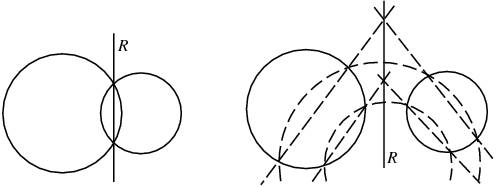
\includegraphics[width=0.5\textwidth]{radical}
\end{center} \end{figure}

\begin{exercise}
Considering the definition of orthogonal circles above, prove that a radical axis is indeed a set of centers of all circles that are orthogonal to $k, l$.
\end{exercise}


\begin{Theorem}[Radical axis theorem]
Let there three circles $a,b,c$ given such that no two are concentric. The three radical axes (for each pair of circles) intersect in a single point called the \emph{radical center}, or are parallel. \\
This also means that there is a unique circle with its center at the radical center that is orthogonal to all three circles. 
\end{Theorem}

\begin{proof}
Consider radical axes $R_{a,b}, R_{b,c}$ intersecting in point $C$. By definition of a radical axis the tangents to $a$ and $b$ through $C$ are equal in length, as well as tangents to $b$ and $c$ through $C$ are. By the transitivity of equality, also tangents to $a$ and $c$ through $C$ are equal in length, which means that $C$ also lies on $R_{a,c}$.
\end{proof}

\begin{figure}[h] \begin{center}
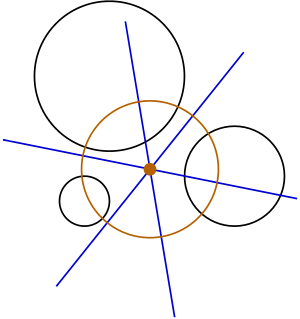
\includegraphics[width=0.5\textwidth]{center}
\end{center} \end{figure}


\begin{exercise}
Prove by similar argument that the unique circle orthogonal to all three circles is indeed centered in radical center.
\end{exercise}

\noindent Let's finish the theory section by mentioning that radical lines play important role in solution of a Problem of Apollonius \footnote{Given three objects, each of which may be a point, line, or circle, draw a circle that is tangent to each}.

\section{Problems}


\begin{enumerate}
\subsection*{Easy}
    \item{Prove that a convex quadrilateral $ABCD$ with $M = AC \cap BD$ is cyclic if and only if $|MA|\cdot|MC| = |MB|\cdot|MD|$.}
    
    \item{Given line segments of lenghts $x$ and $y$, construct a line segment of length $\sqrt{xy}$.}

	\item{We are given line $p$ and points $A$ and $B$ on the same side of $p$ but not on $p$. How can we construct circle tangent to $p$ through points $A$ and $B$?}
	
		\item{We're given two circles with a common tangent line. Let the tangent points be $A$ and $B$. Show that chordal of the two circles divides $AB$ in half.}
		
		\item{Prove that all three altitudes of a triangle intersect in a single point.}
	
\subsection*{Medium}

	\item{We are given line $p$ and points $A$ and $B$ on the opposite sides of $p$. Find circle through $A$ and $B$, such that the length of $p$ inside the circle is minimal.}

	\item{Let $ABCD$ be a quadrilateral with $AB \parallel CD$, $AB > CD$, $AC \perp BD$. Let $O$ be circumcenter of $\triangle ABC$ and $E = OB \cap CD$. Show that $BC^2 = CD \cdot CE$.}
	
	\item{On lines $CA$ and $CB$ of acute triangle $ABC$ there are points $X$ and $Y$. Let $P$ be intersection of $AX$ and $BY$ and $Q$ be intersection of circumcircles of triangles $AXC$ and $BYC$ (other than $C$). Prove that $C$, $P$, and $Q$ are on a line if and only if $ABXY$ is cyclic.}
	
	\subsection*{Difficult}
	
	\item{$ABC$ is an acute triangle and $H$ its orthocenter. Circle with diameter $AH$ intersects circumcircle in points $A$ and $K$. Line $KH$ intersects $BC$ in $M$. Prove that $M$ is midpoint of $BC$.}
	
	\item{Let circles $k$ and $l$ be externaly tangent at point $T$. Let $P$ be any point on $l$. Tangent lines to $k$ through $P$ intersect $k$ at $A$ and $B$. Let $AT \cap l = C$ and $BT \cap l = D$. Let $t$ be tangent to $l$ at $P$ and $M = t \cap CD$. Find set of all possible positions of $M$ as we move $P$ along $l$.}
	
	\item{On lines $AB$ and $AC$ of acute triangle $ABC$ there are points $M$ and $N$. Circles with diameters $BN$, $CM$ intersect at $P$ and $Q$. Prove that $P$, $Q$, and orthocenter $H$ are colinear.}

\end{enumerate}

\begin{thebibliography}{9}
\bibitem{KMS} Ondrej Budáč, Tomáš Jurík, and Ján Mazák. 
	\emph{Zbierka úloh KMS}. Trojsten, Bratislava, 2010.
	
\bibitem{PraSe} Matematický korespondenční seminář. Knihovna. [ONLINE] Available at: \texttt{https://mks.mff.cuni.cz/library/library.php}. [Accessed November 10].
\end{thebibliography}
\end{document}
